%% For double-blind review submission, w/o CCS and ACM Reference (max submission space)
\documentclass[10pt, sigplan]{acmart}
%%\settopmatter{printfolios=true,printccs=false,printacmref=false}
%% For double-blind review submission, w/ CCS and ACM Reference
%\documentclass[sigplan,10pt,review,anonymous]{acmart}\settopmatter{printfolios=true}
%% For single-blind review submission, w/o CCS and ACM Reference (max submission space)
%\documentclass[sigplan,10pt,review]{acmart}\settopmatter{printfolios=true,printccs=false,printacmref=false}
%% For single-blind review submission, w/ CCS and ACM Reference
%\documentclass[sigplan,10pt,review]{acmart}\settopmatter{printfolios=true}
%% For final camera-ready submission, w/ required CCS and ACM Reference
%\documentclass[sigplan,10pt]{acmart}\settopmatter{}


%% Conference information
%% Supplied to authors by publisher for camera-ready submission;
%% use defaults for review submission.
%\acmConference[PL'17]{ACM SIGPLAN Conference on Programming Languages}{January 01--03, 2017}{New York, NY, USA}
%\acmYear{2017}
%\acmISBN{} % \acmISBN{978-x-xxxx-xxxx-x/YY/MM}
%\acmDOI{} % \acmDOI{10.1145/nnnnnnn.nnnnnnn}
%\startPage{1}

%% Copyright information
%% Supplied to authors (based on authors' rights management selection;
%% see authors.acm.org) by publisher for camera-ready submission;
%% use 'none' for review submission.
\setcopyright{none}
%\setcopyright{acmcopyright}
%\setcopyright{acmlicensed}
%\setcopyright{rightsretained}
%\copyrightyear{2017}           %% If different from \acmYear

%% Bibliography style
\bibliographystyle{ACM-Reference-Format}
%% Citation style
%\citestyle{acmauthoryear}  %% For author/year citations
\citestyle{acmnumeric}     %% For numeric citations
%\setcitestyle{nosort}      %% With 'acmnumeric', to disable automatic
                            %% sorting of references within a single citation;
                            %% e.g., \cite{Smith99,Carpenter05,Baker12}
                            %% rendered as [14,5,2] rather than [2,5,14].
%\setcitesyle{nocompress}   %% With 'acmnumeric', to disable automatic
                            %% compression of sequential references within a
                            %% single citation;
                            %% e.g., \cite{Baker12,Baker14,Baker16}
                            %% rendered as [2,3,4] rather than [2-4].


%%%%%%%%%%%%%%%%%%%%%%%%%%%%%%%%%%%%%%%%%%%%%%%%%%%%%%%%%%%%%%%%%%%%%%
%% Note: Authors migrating a paper from traditional SIGPLAN
%% proceedings format to PACMPL format must update the
%% '\documentclass' and topmatter commands above; see
%% 'acmart-pacmpl-template.tex'.
%%%%%%%%%%%%%%%%%%%%%%%%%%%%%%%%%%%%%%%%%%%%%%%%%%%%%%%%%%%%%%%%%%%%%%


%% Some recommended packages.
\usepackage{booktabs}   %% For formal tables:
                        %% http://ctan.org/pkg/booktabs
\usepackage{subcaption} %% For complex figures with subfigures/subcaptions
                        %% http://ctan.org/pkg/subcaption
\usepackage{xspace}
\usepackage{graphicx}
\usepackage{ifthen}
\usepackage{pgfplots}
\usepackage{listings}
\usepgfplotslibrary{statistics}
%



% Source Code
%\usepackage{color}
%\usepackage{textcomp}
%\usepackage{listings}
%\usepackage{ulem}
%\usepackage[T1]{fontenc}
%\usepackage{times}
% \usepackage{needspace}
 

% Source Code
\usepackage{color}
\usepackage{textcomp}
\usepackage{listings}

\definecolor{source}{gray}{0.85}% my comment style
\newcommand{\myCommentStyle}[1]{{\footnotesize\sffamily\color{gray!100!white} #1}}
%\newcommand{\myCommentStyle}[1]{{\footnotesize\sffamily\color{black!100!white} #1}}

% my string style
\newcommand{\myStringStyle}[1]{{\footnotesize\sffamily\color{violet!100!black} #1}}
%\newcommand{\myStringStyle}[1]{{\footnotesize\sffamily\color{black!100!black} #1}}

% my symbol style
\newcommand{\mySymbolStyle}[1]{{\footnotesize\sffamily\color{violet!100!black} #1}}
%\newcommand{\mySymbolStyle}[1]{{\footnotesize\sffamily\color{black!100!black} #1}}

% my keyword style
\newcommand{\myKeywordStyle}[1]{{\footnotesize\sffamily\color{green!70!black} #1}}
%\newcommand{\myKeywordStyle}[1]{{\footnotesize\sffamily\color{black!70!black} #1}}

% my global style
\newcommand{\myGlobalStyle}[1]{{\footnotesize\sffamily\color{blue!100!black} #1}}
%\newcommand{\myGlobalStyle}[1]{{\footnotesize\sffamily\color{black!100!black} #1}}

% my number style
\newcommand{\myNumberStyle}[1]{{\footnotesize\sffamily\color{brown!100!black} #1}}
%\newcommand{\myNumberStyle}[1]{{\footnotesize\sffamily\color{black!100!black} #1}}

\lstset{
language={},
% characters
tabsize=3,
escapechar={!},
keepspaces=true,
breaklines=true,
alsoletter={\#},
literate={\$}{{{\$}}}1,
breakautoindent=true,
columns=fullflexible,
showstringspaces=false,
% background
frame=single,
aboveskip=1em, % automatic space before
framerule=0pt,
basicstyle=\footnotesize\sffamily\color{black},
keywordstyle=\myKeywordStyle,% keyword style
commentstyle=\myCommentStyle,% comment style
frame=single,%
backgroundcolor=\color{source},
% numbering
stepnumber=1,
numbersep=10pt,
numberstyle=\tiny,
numberfirstline=true,
% caption
captionpos=b,
% formatting (html)
moredelim=[is][\bfseries]{<b>}{</b>},
moredelim=[is][\textit]{<i>}{</i>},
moredelim=[is][\underbar]{<u>}{</u>},
moredelim=[is][\color{red}\uwave]{<wave>}{</wave>},
moredelim=[is][\color{red}\sout]{<del>}{</del>},
moredelim=[is][\color{blue}\underbar]{<ins>}{</ins>},
% smalltalk stuff
morecomment=[s][\myCommentStyle]{"}{"},
%    morecomment=[s][\myvs]{|}{|},
morestring=[b][\myStringStyle]',
moredelim=[is][]{<sel>}{</sel>},
moredelim=[is][]{<rcv>}{</rcv>},
moredelim=[is][\itshape]{<symb>}{</symb>},
moredelim=[is][\scshape]{<class>}{</class>},
morekeywords={true,false,nil,self,super,thisContext},
identifierstyle=\idstyle,
}

\makeatletter
\newcommand*\idstyle[1]{%
\expandafter\id@style\the\lst@token{#1}\relax%
}
\def\id@style#1#2\relax{%
\ifnum\pdfstrcmp{#1}{\#}=0%
% this is a symbol
\mySymbolStyle{\the\lst@token}%
\else%
\edef\tempa{\uccode`#1}%
\edef\tempb{`#1}%
\ifnum\tempa=\tempb%
% this is a global
\myGlobalStyle{\the\lst@token}%
\else%
\the\lst@token%
\fi%
\fi%
}
\makeatother


%\newcommand{\ct}{\lstinline[backgroundcolor=\color{white}]}
%\newcommand{\needlines}[1]{\Needspace{#1\baselineskip}}
\newcommand{\lct}{\texttt}

\lstnewenvironment{code}{%
    \lstset{%
    % frame=lines,
    frame=single,
    framerule=0pt,
    mathescape=false
    }%
    \noindent%
    \minipage{\linewidth}%
}{%
    \endminipage%
}%


\lstnewenvironment{codeWithLineNumbers}{%
    \lstset{%
    % frame=lines,
    frame=single,
    framerule=0pt,
    mathescape=false,
    numbers=left
    }%
    \noindent%
    \minipage{\linewidth}%
}{%
    \endminipage%
}%



\newenvironment{codeNonSmalltalk}
{\begin{alltt}\sffamily}
{\end{alltt}\normalsize}



\usepackage{xcolor}
\newcommand{\sd}[1]{\color{red}\fbox{\bfseries\sffamily\scriptsize Stef:}{\sf\small$\blacktriangleright$\textit{#1}$\blacktriangleleft$}\color{black}}
\newcommand{\sk}[1]{\color{blue}\fbox{\bfseries\sffamily\scriptsize Sophie:}{\sf\small$\blacktriangleright$\textit{#1}$\blacktriangleleft$}\color{black}}
\newcommand{\cba}[1]{\color{purple}\fbox{\bfseries\sffamily\scriptsize Clement:}{\sf\small$\blacktriangleright$\textit{#1}$\blacktriangleleft$}\color{black}}
\newcommand*\rot{\rotatebox{90}}




% Source Code
%\usepackage{color}
%\usepackage{textcomp}
%\usepackage{listings}
%\usepackage{ulem}
%\usepackage[T1]{fontenc}
%\usepackage{times}
% \usepackage{needspace}
 

% Source Code
\usepackage{color}
\usepackage{textcomp}
\usepackage{listings}

\definecolor{source}{gray}{0.85}% my comment style
\newcommand{\myCommentStyle}[1]{{\footnotesize\sffamily\color{gray!100!white} #1}}
%\newcommand{\myCommentStyle}[1]{{\footnotesize\sffamily\color{black!100!white} #1}}

% my string style
\newcommand{\myStringStyle}[1]{{\footnotesize\sffamily\color{violet!100!black} #1}}
%\newcommand{\myStringStyle}[1]{{\footnotesize\sffamily\color{black!100!black} #1}}

% my symbol style
\newcommand{\mySymbolStyle}[1]{{\footnotesize\sffamily\color{violet!100!black} #1}}
%\newcommand{\mySymbolStyle}[1]{{\footnotesize\sffamily\color{black!100!black} #1}}

% my keyword style
\newcommand{\myKeywordStyle}[1]{{\footnotesize\sffamily\color{green!70!black} #1}}
%\newcommand{\myKeywordStyle}[1]{{\footnotesize\sffamily\color{black!70!black} #1}}

% my global style
\newcommand{\myGlobalStyle}[1]{{\footnotesize\sffamily\color{blue!100!black} #1}}
%\newcommand{\myGlobalStyle}[1]{{\footnotesize\sffamily\color{black!100!black} #1}}

% my number style
\newcommand{\myNumberStyle}[1]{{\footnotesize\sffamily\color{brown!100!black} #1}}
%\newcommand{\myNumberStyle}[1]{{\footnotesize\sffamily\color{black!100!black} #1}}

\lstset{
language={},
% characters
tabsize=3,
escapechar={!},
keepspaces=true,
breaklines=true,
alsoletter={\#},
literate={\$}{{{\$}}}1,
breakautoindent=true,
columns=fullflexible,
showstringspaces=false,
% background
frame=single,
aboveskip=1em, % automatic space before
framerule=0pt,
basicstyle=\footnotesize\sffamily\color{black},
keywordstyle=\myKeywordStyle,% keyword style
commentstyle=\myCommentStyle,% comment style
frame=single,%
backgroundcolor=\color{source},
% numbering
stepnumber=1,
numbersep=10pt,
numberstyle=\tiny,
numberfirstline=true,
% caption
captionpos=b,
% formatting (html)
moredelim=[is][\bfseries]{<b>}{</b>},
moredelim=[is][\textit]{<i>}{</i>},
moredelim=[is][\underbar]{<u>}{</u>},
moredelim=[is][\color{red}\uwave]{<wave>}{</wave>},
moredelim=[is][\color{red}\sout]{<del>}{</del>},
moredelim=[is][\color{blue}\underbar]{<ins>}{</ins>},
% smalltalk stuff
morecomment=[s][\myCommentStyle]{"}{"},
%    morecomment=[s][\myvs]{|}{|},
morestring=[b][\myStringStyle]',
moredelim=[is][]{<sel>}{</sel>},
moredelim=[is][]{<rcv>}{</rcv>},
moredelim=[is][\itshape]{<symb>}{</symb>},
moredelim=[is][\scshape]{<class>}{</class>},
morekeywords={true,false,nil,self,super,thisContext},
identifierstyle=\idstyle,
}

\makeatletter
\newcommand*\idstyle[1]{%
\expandafter\id@style\the\lst@token{#1}\relax%
}
\def\id@style#1#2\relax{%
\ifnum\pdfstrcmp{#1}{\#}=0%
% this is a symbol
\mySymbolStyle{\the\lst@token}%
\else%
\edef\tempa{\uccode`#1}%
\edef\tempb{`#1}%
\ifnum\tempa=\tempb%
% this is a global
\myGlobalStyle{\the\lst@token}%
\else%
\the\lst@token%
\fi%
\fi%
}
\makeatother


%\newcommand{\ct}{\lstinline[backgroundcolor=\color{white}]}
%\newcommand{\needlines}[1]{\Needspace{#1\baselineskip}}
\newcommand{\lct}{\texttt}

\lstnewenvironment{code}{%
    \lstset{%
    % frame=lines,
    frame=single,
    framerule=0pt,
    mathescape=false
    }%
    \noindent%
    \minipage{\linewidth}%
}{%
    \endminipage%
}%


\lstnewenvironment{codeWithLineNumbers}{%
    \lstset{%
    % frame=lines,
    frame=single,
    framerule=0pt,
    mathescape=false,
    numbers=left
    }%
    \noindent%
    \minipage{\linewidth}%
}{%
    \endminipage%
}%



\newenvironment{codeNonSmalltalk}
{\begin{alltt}\sffamily}
{\end{alltt}\normalsize}



\begin{document}

%% Title information
\title[Assessing primitives performance on multi-stage execution]{Assessing primitives performance\\ on multi-stage execution}       

%% Author with single affiliation.
\author{Sophie Kaleba}
                                        %% can be repeated if necessary
\affiliation{
  %\position{Position1}
  \department{RMoD}              %% \department is recommended
  \institution{Inria}            %% \institution is required
 % \streetaddress{Street1 Address1}
  \city{Lille}
  %\state{France}
  %\postcode{Post-Code1}
  \country{France}                    %% \country is recommended
}
\email{sophie.kaleba@etudiant.univ-lille1.fr}          %% \email is recommended

%% Author with two affiliations and emails.
\author{Cl\'ement B\'era}
\affiliation{
  % \position{}
	\department{Software Languages Lab}              %% \department is recommended
	\institution{Vrije Universiteit Brussel}            %% \institution is required
	\city{Brussel}
  % \state{}
  % \postcode{}
	\country{Belgium}                    %% \country is recommended
}
\email{clement.bera@vub.ac.be}          %% \email is recommended

%% Author with two affiliations and emails.
\author{St\'ephane Ducasse}
\affiliation{
 % \position{Position2b}
  \department{RMoD}             %% \department is recommended
  \institution{Inria}           %% \institution is required
  %\streetaddress{Street3b Address2b}
  \city{Lille}
  %\state{State2b}
  %\postcode{Post-Code2b}
  \country{France}                   %% \country is recommended
}
\email{stephane.ducasse@inria.fr}         %% \email is recommended


%% Abstract
%% Note: \begin{abstract}...\end{abstract} environment must come
%% before \maketitle command
\begin{abstract}

Virtual machines, besides the interpreter and just-in-time compiler optimization facilities, also include a set of primitive operations that the client language can use. Some of these are essential and cannot be performed in any other way. Others are optional, they can be expressed in the client language but are often implemented in the virtual machine to improve performance when the just-in-time compiler is unable to do so (start-up performance, speculative optimizations not implemented or not mature enough, etc.).

In a hybrid runtime, where code is executed by an interpreter and a just-in-time compiler, the implementor can choose to implement optional primitives in the client language, in the virtual machine implementation language (typically C or C++) or on top of the just-in-time compiler back-end. We implemented the String comparison optional primitive in each case. This paper describes the different implementations and compares the execution time in Cog, a Smalltalk virtual machine. 

The paper shows that the implementation with the most reliable and high performance is also the most complex and difficult to implement. Since hundreds of optional primitives can be available, the virtual machine implementor has to carefully choose how to implement each of them to balance between maintenance cost and high performance.

\end{abstract}

%% 2012 ACM Computing Classification System (CSS) concepts
%% Generate at 'http://dl.acm.org/ccs/ccs.cfm'.
%\begin{CCSXML}
%<ccs2012>
%<concept>
%<concept_id>10011007.10011006.10011008</concept_id>
%<concept_desc>Software and its engineering~General programming languages</concept_desc>
%<concept_significance>500</concept_significance>
%</concept>
%<concept>
%<concept_id>10003456.10003457.10003521.10003525</concept_id>
%<concept_desc>Social and professional topics~History of programming languages</concept_desc>
%<concept_significance>300</concept_significance>
%</concept>
%</ccs2012>
%\end{CCSXML}

%\ccsdesc[500]{Software and its engineering~General programming languages}
%\ccsdesc[300]{Social and professional topics~History of programming languages}
%% End of generated code


%% Keywords
%% comma separated list
\keywords{Just-in-Time compiler, Primitive, Virtual machine, Managed runtime}  %% \keywords are mandatory in final camera-ready submission


%% \maketitle
%% Note: \maketitle command must come after title commands, author
%% commands, abstract environment, Computing Classification System
%% environment and commands, and keywords command.
\maketitle


\section{Introduction}
\label{sec:intro}

High level object oriented programming languages are often implemented on top of a virtual machine (VM). As VMs has become more popular, different techniques have been set-up using Just-In-Time (JIT) compilation to improve the overall performance of the runtime such as method JITs \cite{ursPHD} which usually compile methods to native code and tracing JITs \cite{Dynamo, PyPyTracing} which usually compile linear traces of execution into native code. 

On top of its virtual machine, the client language can use a set of \emph{primitives}~\footnote{We use in the paper the Smalltalk terminology (primitive) as this is the programming language used for our evaluation. Some other programming languages, such as Javascript, prefer to use the term built-in instead of primitive.}, which are performed directly by the interpreter rather than by evaluating expressions in a method. We distinguish two kinds of primitives:
\begin{itemize}
	\item \emph{Essential primitives} cannot be performed in any other way. A high-level object oriented language without primitives can move values from one variable to another, but cannot add two integers together. Many arithmetic and comparison operations between numbers are primitives. Some primitives allow to communicate with I/O devices such as the disk, the display and the keyboard. 
	\item \emph{Optional primitives} exist only to make the system run faster. They can be implemented in the client language directly, making its implementation as a primitive optional, but they are implemented in the VM to improve performance.
\end{itemize}

The implementation of an optional primitive in the VM rather than the client language improves performance but also often increases the implementation engineering cost. For example, accessing objects in the VM usually requires some understanding of the memory layout or implementation details, which are not needed in the client language. 

For this reason, some virtual machine implementors attempted to remove most or all optional primitives. Their goal was to improve the execution of the client language with a JIT performing speculative optimizations \cite{ursPHD} for the execution of the optional primitives implemented in the client language to be as fast as the performance of the same primitives written in the VM. Self \cite{ursPHD} and Strongtalk \cite{Strongtalk} were \sk{the?} to first to try this approach. Early versions of the Javascript engine V8 \cite{V8} also implemented most of the primitives, including for example Array operations in Javascript itself. However, without optional primitives implemented in the VM, several problems rise:
\begin{itemize}
	\item High performance relies on a JIT with speculative optimizations, which is hard to implement, maintain and evolve,
	\item The performance of the code not yet optimized is much worse than the peak performance code,
	\item Even mature JIT fail to optimize some narrow cases, where the performance is drastically slower.
\end{itemize}
Overall, this approach requires high engineering time to get a mature optimizing JIT with speculative optimizations and even then, it leads in practice to unreliable performance. 

VMs are traditionally implemented in a low-level language such as C or C++. To balance between memory footprint, start-up performance and peak performance, the execution of code is usually done through multiple execution tiers: the first few executions of a code snippet are done through an interpreter and the JIT compiler at runtime the frequently used code snippets for further executions to be performed quicker. This leads to annoying concerns: for example, let's say we implement a primitive in C. Frequently used portion of code calling that primitive are going to be compiled to native code by the JIT. This is problematic since the native code generated by the JIT is not directly compatible with native code generated by the C compiler: a call from one to another may require to edit the stack pointer and the frame pointer from the client stack to the C stack and to spill or move multiple registers. Switching between both can waste up to around a dozen native instructions. If the primitive is going to execute many instructions, the switch overhead might be negligible, but if the primitive executes only a few instructions, the overhead can be noticeable.

In this paper, we take the example of a string comparison optional primitive. The primitive compares two strings and answers if one string is greater, equal or lower than the other string. The exact specifications are detailed in Section \ref{subsec:primSpec}. We implemented a first version in Smalltalk. We then implemented multiple version compiling through C compilers to native code, using different part of our VM infrastructure. Lastly, we implemented a version in the back-end of the JIT. Each time, we tried to write the code in the most efficient way possible. Then, we compared the execution time of all versions, showing that overall the most complex implementation is the fastest to execute.

Section \ref{sec:implContext} describes our implementation context, \emph{i.e.,} the execution model of the VM we used for our evaluation, how it executes primitives and the specification of our string comparison primitive. Section \ref{sec:implem} details the various implementations of the primitive we used for the evaluation. In Section \ref{sec:eval}, we evaluate the performance of the different implementations with different C compilers and string sizes. We also show the native code of the performance critical part of the primitive generated by each version and discuss it. Further sections compare our work to related works, discuss future work and conclude.

\section{Implementation context}
\label{sec:implContext}

Our evaluation is based on the Cog VM a Smalltalk virtual machine. The Cog VM is based on Dan Ingalls' Smalltalk VM \cite{BackToTheFuture} and have been enhanced with a JIT \cite{CogJIT} compiling one method or closure at a time to native code. Historically, the VM implemented a 32-bits adaptation of the Smalltalk-80 specifications \cite{blueBook}, but the Cog VM is now the default VM for multiple programming languages such as Pharo \cite{PharoByExample}, Squeak \cite{SqueakByExample} and Newspeak \cite{NewspeakOopsla}. 

Section \ref{sec:VMCompil} describes briefly the implementation languages and compilation process of the Cog VM. Section \ref{sec:VMexec} explains briefly the hybrid execution model with an interpreter and a JIT. In Section \ref{sec:primExec}, we detail how primitives are executed. Section \ref{subsec:primSpec} discusses the specifications of the string comparison primitive used for our evaluation.

\subsection{VM compilation}
\label{sec:VMCompil}

Most of the Cog VM code base is written in Slang, a subset of Smalltalk. Slang is compiled to C and then to native code through standard C compilers. The execution engine (the memory manager, the interpreter and the baseline JIT) are entirely written in Slang. The two main purposes of using slang code over plain C are:
\begin{itemize}
	\item to specify with annotations what function needs to be inlined or duplicated with constant parameters, and
	\item to be able to simulate VM execution, executing the Slang code as Smalltalk code on top of a compiled VM for debugging purposes.
\end{itemize}

\begin{figure}[bth]
		\centering
		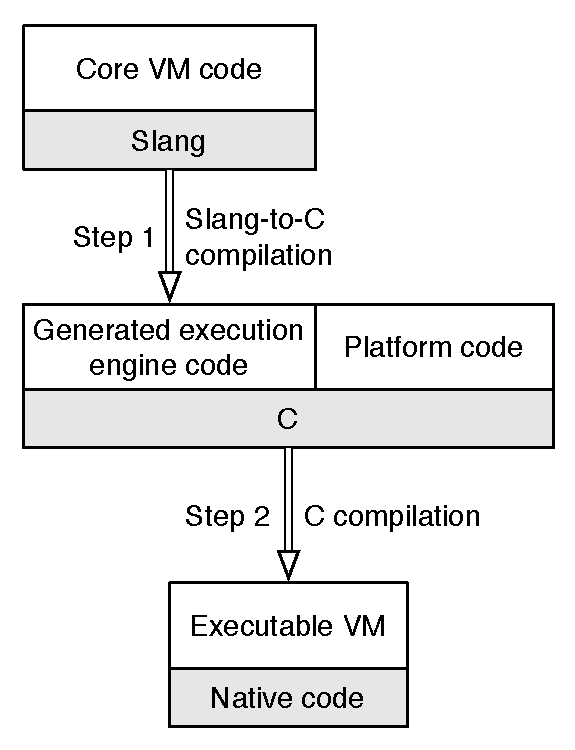
\includegraphics[width=0.6\linewidth]{figures/VMCompilation}
		\caption{Cog VM compilation}
		\label{fig:VMCompilation}
\end{figure}

The executable is generated in two steps as shown on Figure \ref{fig:VMCompilation}, similarly to the RPython toolchain \cite{RPythonToolchain}. The first step is to generate the two C files representing the whole execution engine written in Slang using the Slang-to-C compiler. During the second step, a C compiler is called to compile the execution engine and the platform-specific code written directly in C to the executable VM.

\subsection{VM execution}
\label{sec:VMexec}

The Cog VM executes the client's code using an hybrid runtime with an interpreter and a JIT. The interpreter uses a global look-up cache to speed-up virtual calls. On cache hits, it requests the JIT to compile that method and the native code version is used instead. In most case, the JIT is used at the second activation of the method. Closures have similar heuristics.

The VM code, including the interpreter code, is compiled by a C compiler and uses the C stack at runtime. During its execution, the interpreter modifies the execution stack of the client language, which is different from its own code stack as shown on Figure \ref{fig:TwoStacks}. This means for example that the frame pointer register in the processor refers to a stack frame on the C stack and that a processor push instruction pushes a value on the C stack. When executing the native code generated by JIT, only the client language stack is used. This means for example that the frame pointer register in the processor refers to a stack frame on the client stack and that a processor push instruction pushes a value on the client stack.

\begin{figure}[tbh]
		\centering
		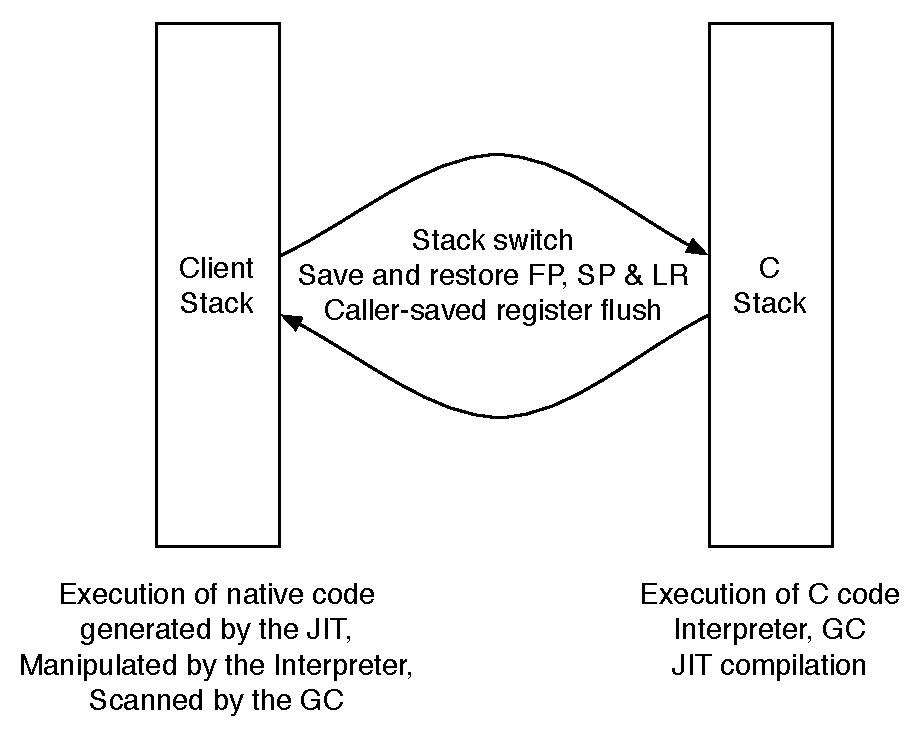
\includegraphics[width=0.99\linewidth]{figures/TwoStacks}
		\caption{Client and C stacks}
		\label{fig:TwoStacks}
\end{figure}

Because of this design, switching the execution between the interpreter and the native code generated by the JIT has a cost. Effectively, the VM needs to switch the frame pointer, the stack pointer and depending on architecture the link register from one stack to the other one. It also needs to save those pointers to be able to resume execution from one stack to the other one. In addition, caller-saved registers on the C conventions or the JIT convention need to be saved since the VM cannot tell ahead what code is going to be used in the other execution model and what registers are required. We estimate the overhead to up to around a dozen of processor instruction, the exact number varies a lot so it is difficult to precise it (the number of register to edit depends on the processor and on the code executed).

Most of the primitives are implemented either in Slang or directly in C. They benefit from the C compiler optimizations to be efficient. When called from the interpreter, activating a primitive is just a C call (the primitive function pointer is cached in the look-up cache next to the method to activate). When called from the native code generated by the JIT, activating a primitive requires to switch the execution from the client stack to the C stack, perform the primitive, and switch back to resume execution. If the primitive takes a significant amount of instructions to execute, for example, the primitive is copying 100kb from one array to another one, the stack switch dance overhead is negligible. If the primitive is very quick to perform, for example, the primitive is adding two integers which do not overflow, the overhead is massive: the execution cost of the addition goes from a few processor instructions to a few dozen instructions.

To solve this performance bottleneck, the Cog VM allows to redefine primitives in Cog's Register Transfer Language (RTL), an abstract assembly which is compiled to native code through Cog's JIT back-end. Such primitives are then generated to native code at runtime when a method annotated with the primitive is compiled to native code. This allows the primitive to be performed in the client stack with the client calling convention, saving register moves and the stack switch dance. Primitives redefined in such way can be entirely or partially redefined. In the later case, only the common cases are re-implemented on top of the JIT back-end, and an unimplemented case happens at runtime, the generated native code calls the C primitive instead, adding overhead only in uncommon cases. 

\subsection{Primitive execution}
\label{sec:primExec}

In the Cog VM, primitives are always associated with compiled methods. A compiled method has information in its header to inform the virtual machine if it has a primitive operation or not. When activating a method with a primitive, the primitive function is executed before the method's bytecode. If the primitive succeeds, the primitive returns a result, as if it were the result of the virtual call. If the primitive fails, it does so without side-effects and execution continues executing the method's bytecode, as if the primitive had not been present.

To fail without side-effects a primitive must validate any parameters and any state fetched from them, before changing execution state by performing its operations. Validation involves any of testing for a specific class, testing for bit vs pointer objects, bounds checks, and recursively applying these tests to substructure of the parameters. For example, the primitive that installs a cursor examines the first parameter to check that it represents a valid cursor object, comprised of two bitmaps, one for the image and one for the shape, plus a point to specify the cursor's hotspot. 

\subsection{String comparison primitive}
\label{subsec:primSpec}

\cba{Cette partie je faisais la queue dans la gare en mm temps, a relire}
 
 The primitive specification is a bit tedious to explain, since as we were trying to improve its performance, we had to change the specifications. In this section we describe first the string implementation, then the original primitive specification and why they were problematic and lastly the new specifications.
 
\paragraph{String representations.} Strings are represented in all programming languages on top of the Cog VM in two possible forms, ByteStrings and WideStrings. ByteStrings encode each character of the string in a single byte. The encoding usually follows the extended ASCII standard. WideStrings encode each character of the string in 32 bits. The encoding usually follows Unicode specifications. In this paper, we will discuss only the implementation of the string comparison primitive for ByteStrings. WideStrings use an implementation entirely implemented in the client language, and so far, it has not been reported as a performance bottleneck for any program of any users. To sort arrays of strings, strings can be compared. They can be compared in the default order (ASCII or Unicode) or using different orders, for example, the case insensitive order.
 
\paragraph{Original specification.}  The original primitive took three operands. The two first operands were the two ByteStrings to compare and the third operand is the order table, a ByteArray encoding the order of characters. The default order is the ASCII order, hence each entry corresponds to its index in the byte array (The ByteArray has a size of 256, and accessing the element i, with 0 <= i <= 255, answered i). However, in some case, the program may do case insensitive ByteStrings comparison. In this case, the order ByteArray is different, since some entries answer the same value (for example, the entry for the 41 and 61, respectively characters A and a, both answer the same value). To compare the two ByteStrings, the primitive conceptually iterates byte by byte over the two objects until it reaches the end of one them, comparing for each byte that the value present in the order ByteArray at the index is greater, equal or smaller than the value computed from the other ByteString. If a difference is met, the value returns based on the result, if not, at the end of the iteration the primitive compares the ByteString sizes and returns. Based on the three parameters, the primitive answered 3,2 or 1 depending if the first ByteString was greater, equal or smaller than the second one.
 
\paragraph{Specification issues.} As we were trying to optimize string comparison but specifically string equality, we encountered two main issues:
\begin{itemize}
	\item \emph{Returned value:} Other programming languages implement the primitive to return a negative integer, 0 or a positive integer instead of 1,2 or 3. It looks like a minor difference, but it is quite important for performance. With a negative, 0 or positive value, the primitive can just answer the difference between two different characters or the difference in size if all first characters are equal. With 1,2 or 3, the primitive has to end with multiple branches to know what number to return. In native code, a subtraction is on common architecture quicker to perform than one or multiple branches. In addition, the primitive code is easier to write with the subtraction when writing directly the assembly instructions and we did exactly that when writing the primitive on top of the JIT's back-end.
	\item \emph{Order:} Having the order as the third operands is convenient in some cases (case insensitive comparison), but is just overhead in the common case (checking for string equality).
\end{itemize} 
 
\paragraph{Final specification.} The final specification we productized last month takes two or three parameters. The third parameter, the order, is optional. If the third parameter is absent, the VM assumes the byte ordering (ASCII order) is the order to compare against. Therefore, the VM does not need to go through the indirection order array in the common case. The primitive answers a negative value if the first parameter is smaller than the second, 0 if they are equal, and a positive value if the first parameter is greater than the second one.
\cba{Maybe rewrite the last paragraph to make it clearer / more formal. - CF Java spec ?}

\section{Different primitive implementations}
\label{sec:implem}
 
 This section first describes the different ways of implementing a primitive. We then explain how each of these version are executed by the VM and the pros and cons of each and every.
 
 \subsection{Different implementations and executions}
 
 \cba{Maybe wrte version A, B, C , D , E or a word to represent what they are (Smalltalk) (SmartSyntax) (Plugin) (Slang) (Slang+JIT)
 so you can refer to that to talk about any of these later and not wirte each time : the implem with ths wirtten that wya and exec that way.
 Myabe those could be paragraph titles instead of the following}
 
\paragraph{Baseline: pure Smalltalk.}
: baseline
Smalltalk code on top of VM. Used as our baseline for benchmarks.

\begin{code}
compareWithPureST: aString 
	
	| c1 c2 length1 length2 |
	length1 := self size.
	length2 := aString size.
		1 to: (length1 min: length2) do: [ :i |
			(c1 := self basicAt: i) = (c2 := aString basicAt: i) 
			ifFalse: [
				c1 < c2
					ifTrue: [ ^1 ]
					ifFalse: [ ^3 ] ] ].
		length1 = length2 ifTrue: [ ^2 ].
		length1 < length2
			ifTrue: [ ^1 ]
			ifFalse: [ ^3 ] 
\end{code}

Expliquer to:do: over do: (to explain expresiveness) => core lib often use to:do: and not do:
New spec

\paragraph{Existing: Smart Syntax Plugin.}
Restricted Smalltalk

written in Smalltalk with restrictions.
Compiled to C AOT into a plugin.
Write once, fall-back + compiled.

old spec

\paragraph{Existing: Slang Plugin.}
Slang, but no access au fonctions de la VM drectement.
 interpreterProxy. (C compiler inlining, linking time ? cmacro ?)
 
 old spec

\paragraph{Pure Slang.}

new spec

\paragraph{Pure Slang with JIT support.}
Cog RTL

generate functions as machine code
partial implementation (frequent cases are implemented)
Sometimes, fallback to less-optimised version

new spec
 
 \subsection{Pros and cons}
 
  Can be changed like Smalltalk code (No C compilation whatsoever). Readability. Only impl without VM recompilation.

Baseline performance is not that great.

Number of implementations to maintain: 1, 2 or 3: same implem for primitive in C and fall back code in Smalltalk, relatively easy to read/code.
recompilation. 
changing the prim => changing all clients (VM compil from Pharo or Squeak different results
Performance: cross file inlining not possible by default. (InterpreterProxy indirection)
Control on generated code => difference LLVM/GCC
 Pure C performance (no interpreter proxy).
 no C-St jump. Control over the outcome (reliable performance)
 costly jumps between Smalltalk and C runtime (trampolines), need to recompile vm sources, little control over outcome (c compilers 
 need to recompile vm sources (trampolines), code readability 
 
 \subsection{Comparison}


\cba{expliquer tableau comparatif}

\begin{table}
\centering
\begin{tabular}{|c||c|c|c|c|}
  \hline
    & \rot{Engineering time} & \rot{Execution time} & \rot{Readability}  \\
  \hline
  Baseline & + & +++ & +++ \\
  SmartSyntax & ++ & ++ & ++ \\
  SlangPlugin & ++ & ++ & ++ \\
  PureSlang & +++ & + & ++ \\
  Slang+JIT & +++ & + & + \\
  \hline
\end{tabular}
\caption{Trade-offs between implementations: synthetized}
\label{tab:comparisontable}
\end{table}


Each of these implementations has its pros and cons considering the context. In the end, there is always a trade-off between engineering time and performance. In 

Trade-off engineering time and performance.
- recompiler la VM ou pas (Plugin externes, code Smalltalk)
- complexite d'implem (comprehension Smalltalk, C, ASM)

\section{Evaluation}
\label{sec:eval}

All these versions of the primitives have been implemented. Compare performances

\subsection{Set-up}
Describe set-up:
GCC eval Ubuntu + machine spec
LLVM eval Mac OS X + machine spec.

\subsection{Micro-benchmarks}

%%%
% Legend definition (so I can change it once for all)
%%%

\def\legBase{Baseline}
\def\legSmartSyntaxPlug{Smart Syntax}
\def\legSlangPlug{Plugin}
\def\legSlang{Pure Slang}
\def\legRTL{Slang+JIT}

%%%
% End Legend
%%%

\begin{figure*}
  \centering
    \begin{subfigure}[b]{\textwidth}
    \begin{subfigure}[b]{.19\textwidth}
    \begin{tikzpicture}
      \begin{axis}
      [
        x=0.5cm,
        xtick={1,...,5},
        xticklabel style={rotate=90},
        bar width=0.3cm,
        enlarge x limits={abs=0.45cm},
        xticklabels={\legBase, \legSmartSyntaxPlug, \legSlangPlug, \legSlang, \legRTL},
        font={\footnotesize},
	ybar=10pt,
	ymin=0
        ]
\addplot[
    fill=black!25,
    %draw=none,
    %fill,
    draw=black,
    fill,
    point meta=y,
    every node near coord/.style={inner ysep=5pt},
    error bars/.cd,
        y dir=both,
        y explicit
]  
table [y error=error] {
x   y           error    
1   1           0 
2   0.3411212   0.0006746299 
3   0.3375418   0.001577878
4   1.077762   0.005363974 
5   2.490423    0.004304882 
};            
      \end{axis}
    \end{tikzpicture}
    \subcaption{Size 0}
    \end{subfigure}
     \begin{subfigure}[b]{.19\textwidth}
    \begin{tikzpicture}
      \begin{axis}
      [
        x=0.5cm,
        xtick={1,...,5},
        xticklabel style={rotate=90},
        bar width=0.3cm,
        enlarge x limits={abs=0.45cm},
        xticklabels={\legBase, \legSmartSyntaxPlug, \legSlangPlug, \legSlang, \legRTL},
        font={\footnotesize},
	ybar=10pt,
	ymin=0
        ]
\addplot[
    fill=black!25,
    %draw=none,
    %fill,
    draw=black,
    fill,
    point meta=y,
    every node near coord/.style={inner ysep=5pt},
    error bars/.cd,
        y dir=both,
        y explicit
]  
table [y error=error] {
x   y           error    
1   1           0 
2   0.3411212   0.0006746299 
3   0.3375418   0.001577878
4   1.077762   0.005363974 
5   2.490423    0.004304882 
};            
      \end{axis}
    \end{tikzpicture}
    \subcaption{Size 1 TO UPDATE}
    \end{subfigure}
    \begin{subfigure}[b]{.19\textwidth}
    \begin{tikzpicture}
      \begin{axis}
      [
        x=0.5cm,
        xtick={1,...,5},
        xticklabel style={rotate=90},
        bar width=0.3cm,
        enlarge x limits={abs=0.45cm},
        xticklabels={\legBase, \legSmartSyntaxPlug, \legSlangPlug, \legSlang, \legRTL},
        font={\footnotesize},
	ybar=10pt,
	ymin=0
        ]
\addplot[
    fill=black!25,
    draw=black,
    point meta=y,
    every node near coord/.style={inner ysep=5pt},
    error bars/.cd,
        y dir=both,
        y explicit
] 
table [y error=error] {
x   y           error    
1   1           0 
2   1.3891212   0.0029489731 
3   1.3149840   0.020471694
4   3.818961   0.054523074 
5   6.740474    0.010805042 
};            
      \end{axis}
    \end{tikzpicture}
    \subcaption{Size 5}
    \end{subfigure}
    \begin{subfigure}[b]{.19\textwidth}
 \begin{tikzpicture}
      \begin{axis}
      [
        x=0.5cm,
        xtick={1,...,5},
        xticklabel style={rotate=90},
        bar width=0.3cm,
        enlarge x limits={abs=0.45cm},
        xticklabels={\legBase, \legSmartSyntaxPlug, \legSlangPlug, \legSlang, \legRTL},
        font={\footnotesize},
	ybar=10pt,
	ymin=0
        ]
\addplot[
    fill=black!25,
    draw=black,
    point meta=y,
    every node near coord/.style={inner ysep=5pt},
    error bars/.cd,
        y dir=both,
        y explicit
] 
table [y error=error] {
x   y           error    
1   1           0 
2   8.6795487   0.0586762222 
3   8.9585208   0.116958804
4   15.809515   0.300447885 
5   16.752667    0.106255682 
};            
      \end{axis}
    \end{tikzpicture}
    \subcaption{Size 100}
    \end{subfigure}
    \begin{subfigure}[b]{.19\textwidth}
     \begin{tikzpicture}
      \begin{axis}
      [
        x=0.5cm,
        xtick={1,...,5},
        xticklabel style={rotate=90},
        bar width=0.3cm,
        enlarge x limits={abs=0.45cm},
        xticklabels={\legBase, \legSmartSyntaxPlug, \legSlangPlug, \legSlang, \legRTL},
        font={\footnotesize},
	ybar=10pt,
	ymin = 0
        ]
\addplot[
    fill=black!25,
    draw=black,
    point meta=y,
    every node near coord/.style={inner ysep=5pt},
    error bars/.cd,
        y dir=both,
        y explicit
] 
table [y error=error] {
x   y           error    
1   1           0 
2   13.6051267   0.0589164968 
3   14.7789145   0.147140189
4   24.417751   0.186326223 
5   24.480071    0.095038374 
};            
      \end{axis}
    \end{tikzpicture}
   \subcaption{Size 1000}
   \end{subfigure}
  % \caption{GCC-Linux results}
   % \label{fig:gcc}
   \subcaption*{\textbf{GCC-Linux results}\vspace{0.3cm}}     
   \end{subfigure}
 \begin{subfigure}[b]{\textwidth}
    \begin{subfigure}[b]{.19\textwidth}
    
    \begin{tikzpicture}
      \begin{axis}
      [
        x=0.5cm,
        xtick={1,...,5},
        xticklabel style={rotate=90},
        bar width=0.3cm,
        enlarge x limits={abs=0.45cm},
        xticklabels={\legBase, \legSmartSyntaxPlug, \legSlangPlug, \legSlang, \legRTL},
        font={\footnotesize},
	ybar=10pt,
	ymin=0
        ]
\addplot[
    fill=black!25,
    draw=black,
    point meta=y,
    every node near coord/.style={inner ysep=5pt},
    error bars/.cd,
        y dir=both,
        y explicit
] 
table [y error=error] {
x   y           error    
1   1           0 
2   0.3147064   0.002288488 
3   0.3035965   0.001786185
4   0.8545431   0.006132950 
5   2.250732    0.04133638 
};            
      \end{axis}
    \end{tikzpicture}

    \subcaption{Size 0}
    \end{subfigure}
     \begin{subfigure}[b]{.19\textwidth}
    
    \begin{tikzpicture}
      \begin{axis}
      [
        x=0.5cm,
        xtick={1,...,5},
        xticklabel style={rotate=90},
        bar width=0.3cm,
        enlarge x limits={abs=0.45cm},
        xticklabels={\legBase, \legSmartSyntaxPlug, \legSlangPlug, \legSlang, \legRTL},
        font={\footnotesize},
	ybar=10pt,
	ymin=0
        ]
\addplot[
    fill=black!25,
    draw=black,
    point meta=y,
    every node near coord/.style={inner ysep=5pt},
    error bars/.cd,
        y dir=both,
        y explicit
] 
table [y error=error] {
x   y           error    
1   1           0 
2   0.3147064   0.002288488 
3   0.3035965   0.001786185
4   0.8545431   0.006132950 
5   2.250732    0.04133638 
};            
      \end{axis}
    \end{tikzpicture}

    \subcaption{Size 1 TO UPDATE}
    \end{subfigure}
    \begin{subfigure}[b]{.19\textwidth}

    \begin{tikzpicture}
      \begin{axis}
      [
        x=0.5cm,
        xtick={1,...,5},
        xticklabel style={rotate=90},
        bar width=0.3cm,
        enlarge x limits={abs=0.45cm},
        xticklabels={\legBase, \legSmartSyntaxPlug, \legSlangPlug, \legSlang, \legRTL},
        font={\footnotesize},
	ybar=10pt,
	ymin=0
        ]
\addplot[
    fill=black!25,
    draw=black,
    point meta=y,
    every node near coord/.style={inner ysep=5pt},
    error bars/.cd,
        y dir=both,
        y explicit
] 
table [y error=error] {
x   y           error    
1   1           0 
2   1.2505193   0.004611354 
3   1.2295801   0.001810171
4   2.8205415   0.008035024 
5   7.089806    0.01403785 
};            
      \end{axis}
    \end{tikzpicture}
    \subcaption{Size 5}
    \end{subfigure}
    \begin{subfigure}[b]{.19\textwidth}
 \begin{tikzpicture}
      \begin{axis}
      [
        x=0.5cm,
        xtick={1,...,5},
        xticklabel style={rotate=90},
        bar width=0.3cm,
        enlarge x limits={abs=0.45cm},
        xticklabels={\legBase, \legSmartSyntaxPlug, \legSlangPlug, \legSlang, \legRTL},
        font={\footnotesize},
	ybar=10pt,
	ymin=0
        ]
\addplot[
    fill=black!25,
    draw=black,
    point meta=y,
    every node near coord/.style={inner ysep=5pt},
    error bars/.cd,
        y dir=both,
        y explicit
] 
table [y error=error] {
x   y           error    
1   1           0 
2   6.6951738   0.062391122 
3   6.6032572   0.024774416
4   10.3029394  0.061481532 
5   17.979611   0.10127936 
};            
      \end{axis}
    \end{tikzpicture}
    \subcaption{Size 100}
    \end{subfigure}
    \begin{subfigure}[b]{.19\textwidth}

    \begin{tikzpicture}
      \begin{axis}
      [
        x=0.5cm,
        xtick={1,...,5},
        xticklabel style={rotate=90},
        bar width=0.3cm,
        enlarge x limits={abs=0.45cm},
        xticklabels={\legBase, \legSmartSyntaxPlug, \legSlangPlug, \legSlang, \legRTL},
        font={\footnotesize},
	ybar=10pt,
	ymin=0
        ]
\addplot[
    fill=black!25,
    draw=black,
    point meta=y,
    every node near coord/.style={inner ysep=5pt},
    error bars/.cd,
        y dir=both,
        y explicit
] 
table [y error=error] {
x   y           error    
1   1           0 
2   9.4064534   0.036698187 
3   9.2138415   0.013982843
4   13.4384830  0.040202717 
5   26.404792   0.09298324 
};            
      \end{axis}
    \end{tikzpicture}
   
   \subcaption{Size 1000}
   \end{subfigure}
   \subcaption*{\textbf{LLVM-Mac results}}
    \end{subfigure}
   \label{fig:llvm}
\end{figure*}


%\cba{Je pense string de taille 0-1 c'est cool pour montrer que le code C va moins vite que pur smalltalk dans ce cas (si c'est vraiment le cas)}
We performed the benchmarks upon 4 different string sizes: 0, 5, 100 and 1000 characters, using 2 different compilers: GCC on one hand and LLVM on the other hand.

The results are shown in terms of relative speed-up towards the baseline implementation, i.e. the pure smalltalk version. 
We can notice some patterns over the results in figures \ref{fig:gcc} and \ref{fig:llvm}:
\begin{itemize}
\item The execution time of the SmartSyntax and Plugin implementations is either very close or greater than the baseline's for the small strings. This can be explained by the high cost of the switching between the C and Smalltalk stacks, as mentionned in \sk{faire ref à la partie}.
\item The Slang+JIT implementation is more performant in every case. Nevertheless, 
the performance gap between this implementation and the PureSlang one tends to decrease as the string size increase. The comparison loop \sk{ref to appendix}
\end{itemize} proves to be more and more time-consuming because of the higher number of iterations.


Howerver, one could notice a rather striking performance difference between the 2 compilers: when compiling with GCC, we notive in Figure \ref{gcc} that the performances between the PureSlang and Slang+JIT implementations are really close for long strings (100 characters and longer), with respectively 24,42 and 24,48 relative speed-up factor for a 1000-characters string. They still greatly differ when LLVM is used, with respectively 13,44 and 26,40 relative speed-up factor.

%\begin{lstlisting}[language={[x64]Assembler}]
%movzbl 0x8(%eax,%edx,1),%ebp
%movzbl 0x8(%eax,%ebx,1),%ecx
%cmp    %ecx,%ebp
%jne    6e8 <primitiveCompareWith+0x1f8>
%add    $0x1,%eax
%cmp    %eax,%edi
%jne    610 <primitiveCompareWith+0x120> 
%\end{lstlisting}


\begin{table}
\centering
\begin{tabular}{|r|l|}
  \hline
   GCC & LLVM  \\
  \hline
  `movzbl 0x8(\%eax,\%edx,1),\%ebp` & `movl -0x14(\%ebp), \%esi`  \\
  movzbl 0x8(\%eax,\%ebx,1),\%ecx & movzbl 0x8(\%edx,\%esi), \%esi \\
  cmp    \%ecx,\%ebp & movl -0x18(\%ebp), \%edi \\
  jne    0x8558 &  movzbl 0x8(\%edx,\%edi), \%edi \\
  add    \$0x1,\%eax & subl \%edi, \%esi \\
  cmp    \%eax,\%edi &  jne 0x1f660 \\
  jne    0x8480 & incl \%edx \\
   & cmpl \%ebx, \%edx \\
   & jl 0x1f644 \\
  \hline
\end{tabular}
\caption{Different compilers optimizations: GCC and LLVM}
\label{tab:cmp_asm}
\end{table}
    
\cba{Show ASM loops and discuss the differences
add appendix with full code}

\subsection{Macro-benchmarks}
Intro sentence with ref to squeak speed center.
JSON

\section{Discussion and related work}

\cba{Maybe talk in those cases the number of representation of the primitives}

We identified two directly related works. In some languages (Strongtalk, Self, RSqueak), the implementors tried to decrease the overall number of optional primitives by improving the client language performance, reducing the need for such primitives \cite{Strongtalk, ursPHD, NoPrimTracing}. In addition, in the V8 project  \cite{V8}, the interpreter was entirely built on top of the V8 JIT's back-end using a specific DSL similar to Cog's RTL.  

\subsection{Decreasing the number of primitives}

The philosophy of Self and Strongtalk, both high performance VMs, were to improve the performance of the client language with a mature optimizing JIT featuring advanced optimizations such as speculative optimizations \cite{Strongtalk, ursPHD}. In this context, the need of primitive is reduced, since the performance gain from using a primitive over the client language is low or inexistant. More recently, Felgentreff \emph{et al.} \cite{NoPrimTracing} analysed the performance difference between primitives implemented in C, RPython, and Smalltalk. They showed that with the RPython toolchain framework, the performance difference between all three implementation was not that big, hence they could choose to implement some optional primitives in the client language over C or RPython without performance drop to reduce the number of primitives to maintain.

These approaches have the advantage of decreasing the primitive maintenance cost since fewer primitives have to be maintained. The performance problem is however partially solved: only the peak performance is similar with and without the primitives. Since those system rely on JITs, start-up performance is worse than peak performance, increasing the performance difference at start-up between the client code and the primitive. In addition, the performance can be  unreliable with optimizing JITs. The implementors of Morphic \cite{MorphicSelf} on top of the Self VM were complaining that changing a single line of code could lead to important performance drop and they would not understand why. Those performance drops were due to the optimizing JIT taking different optimization decisions. This problem was so significant that recently the V8 team \cite{V8} rewrote their primitives written in Javascript (named built-ins in their project) in a DSL compiled ahead of time through their JIT back-end to improve the performance of the primitives and therefore decrease the performance drop between baseline and peak performance. Aside from the start-up performance and the performance unreliability problems described, these approaches also require a mature optimizing JIT, hard to implement and maintain.

\subsection{No stack switch overhead}

To avoid paying the stack switch cost between the client Stack and the C stack, the V8 team recently wrote an interpreter Ignition in a DSL compiled ahead of time through their JIT back-end to native code. With their primtives and their interpreter written in the DSL, the V8 runtime rarely needs to switch between the client and the C stack (no need to switch to interpret code, no need to switch for primitives). In this context, the stack switch overhead is not a problem anymore.

In our context, implementing a similar approach would require us to compile Slang to native code through our JIT compiler back-end or to rewrite the interpreter on top of Cog JIT's RTL. Slang has some abstractions over native code, similarly to C. Compiling Slang ahead of time to native code efficiently requires us to re-implement optimizations implemented in C compilers and we don't want that complexity or to lower the abstractions level of Slang to express native code optimizations, which would increase the complexity of Slang, which we don't want either. Rewriting the interpreter on top of Cog JIT's RTL is possible but requires a significant amount of work. 
	
\section{Future work and conclusion}
1. number of representations\\
2. common representation
\cba{Future work -> primitive processor dependent (i.e. SSE4 instrs), pros and cons and why you did not do it (ingeniering cost per back-end)}
\cba{Inlining in Sista + ref}
\cite{SistaFastStartUp}

Conclusion: trade off expressiveness performance


%% Acknowledgments
%%\begin{acks}                            %% acks environment is optional
                                        %% contents suppressed with 'anonymous'
  %% Commands \grantsponsor{<sponsorID>}{<name>}{<url>} and
  %% \grantnum[<url>]{<sponsorID>}{<number>} should be used to
  %% acknowledge financial support and will be used by metadata
  %% extraction tools.
%  This material is based upon work supported by the
%  \grantsponsor{GS100000001}{National Science
%    Foundation}{http://dx.doi.org/10.13039/100000001} under Grant
%  No.~\grantnum{GS100000001}{nnnnnnn} and Grant
%  No.~\grantnum{GS100000001}{mmmmmmm}.  Any opinions, findings, and
%  conclusions or recommendations expressed in this material are those
%  of the author and do not necessarily reflect the views of the
%  National Science Foundation.
%\end{acks}


%% Bibliography
\bibliography{sista}


%% Appendix
\appendix
\section{Appendix}

\cba{Source code et generated C and ASM code for all versions}

Text of appendix \ldots

\end{document}
